%! program = pdflatex

%\documentclass[12pt,a4paper]{memoir} % for a long document
%\documentclass[12pt,a4paper,article]{memoir} % for a short document
\documentclass[12pt,a4paper,article]{memoir}
\usepackage{geometry}
 \geometry{
 a4paper,
 total={210mm,297mm},
 left=20mm,
 right=20mm,
 top=20mm,
 bottom=20mm,
 }
% \usepackage[titletoc]{appendix}

\usepackage{graphicx}
\usepackage{listings}
\usepackage[dvipsnames]{xcolor}
\usepackage{hyperref}
\usepackage{cleveref}

%\lstset{frame=tb,
%  language=C++,
%  aboveskip=3mm,
%  belowskip=3mm,
%  showstringspaces=false,
%  columns=flexible,
%  basicstyle={\small\ttfamily},
%  numbers=none,
%  numberstyle=\tiny\color{mygray},
%  keywordstyle=\color{blue},
%  commentstyle=\color{mygreen},
%  stringstyle=\color{mymauve},
%  breaklines=true,
%  breakatwhitespace=true,
%  tabsize=2
%}

\definecolor{codegreen}{rgb}{0,0.6,0}
\definecolor{codegray}{rgb}{0.5,0.5,0.5}
\definecolor{codepurple}{rgb}{0.58,0,0.82}
\definecolor{backcolour}{rgb}{0.95,0.95,0.92}
 

\lstdefinestyle{MyCodeStyle} {
%  language=C++, % choose the language of the code
  backgroundcolor=\color{backcolour},
  commentstyle=\color{codegreen},
  keywordstyle=\color{magenta},
  numberstyle=\tiny\color{codegray},
  stringstyle=\color{codepurple},
  basicstyle=\footnotesize,
  breakatwhitespace=false,
  breaklines=true,
  captionpos=b, % sets the caption-position to bottom
  keepspaces=true,                 
  numbers=none, % where to put the line-numbers
  showspaces=false, % show spaces adding particular underscores
  showstringspaces=false, % underline spaces within strings
  showtabs=false, % show tabs within strings adding particular underscores
  frame=single, % adds a frame around the code
  tabsize=2, % sets default tabsize to 2 spaces
  rulesepcolor=\color{blue},
  rulecolor=\color{black},
}

\hypersetup{
    colorlinks,
    citecolor=black,
    filecolor=black,
    linkcolor=black,
    urlcolor=black
}

\graphicspath{ {./img/} }
% See the ``Memoir customise'' template for some common customisations
% Don't forget to read the Memoir manual: memman.pdf

\title{Optimizing Alya simulations of multi-physics problems with Dakota}
\author{Rogeli Grima}
%\date{10/12/2014} % Delete this line to display the current date

% Make appear "Appendix" in the ToC
\renewcommand*{\cftappendixname}{Appendix\space}

%%% BEGIN DOCUMENT
\begin{document}

\maketitle
\tableofcontents*

\chapter{Introduction}

Dakota is a toolkit that provides a flexible, extensible interface between analysis codes and iterative systems analysis methods. It contains algorithms for optimization, uncertainty quantification, parameter estimation and sensitivity/variance analysis.

Alya is a computational method that is used to simulate complex physical systems. On many occasions we want to use these simulations to find an acceptable or optimized solution for a particular system. Dakota will help us to use Alya as a design tool. It will help us to solve very important questions as: What is the best design? How safe is it? How much confidence do I have in my answer?

This user's guide is intended to provide some background information on how to use Dakota to solve optimization problems that involve a simulation with Alya. We assume the user has some familiarity with Alya execution and configuration.

In this guide we will show how to use Dakota in Marenostrum, how to prepare your simulations with Alya, how to process their outputs and we will provide some basic examples.

\section{Dakota workflow}

Before you start working with Dakota and Alya, is important to know the Dakota's workflow. This will give you a better perspective of what is happening.

Dakota receives input and configuration from a variety of text files prepared by the user, and connects to any simulation code by other text files. This simple interface is one of the most important features of Dakota, as it makes it easy to change the iterative method or strategy by just changing a few lines in the Dakota input file.

In Figure \ref{fig:Workflow}, we can see the Dakota workflow. The user should provide an input file to Dakota. This input file controls the algorithm that we want to run, the function to be evaluated, the variables of this function and the outputs that we expect.

\begin{figure}[htb!]
  \centering
    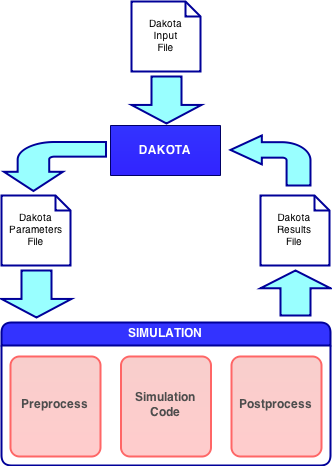
\includegraphics[width=0.4\textwidth]{DakotaWorkflow}
  \caption{Dakota Workflow}
  \label{fig:Workflow}
\end{figure}

Dakota generates a parameter file for every function evaluation. This file contains a specific value of every variable and specifies the kind of returning values that it needs (function evaluation, derivatives or/and second derivatives).

Dakota treats the simulation code as a black box. Most of the codes, like Alya, don't know what to do with the parameter file, so it is common to create a script to connect the simulation code with Dakota. In this script we merge the Dakota parameters file with the simulation code input files. Once we have some proper input files we can run the simulation code, extract the significant data from its output files and post-process that data in order to generate the appropriate objective function and the Dakota results file.

\chapter{Dakota tutorial}
\section{Set up Dakota}

We have installed in Marenostrum the last three versions of Dakota. Althought, most of the experiments that we have ran have been done using version 5.4 we encourage you to use the last version. From now on, all the information that we will provide you in this guide will refer to version 6.1. You can find the several installed versions of Dakota in:

\begin{itemize}
\item /gpfs/projects/bsc21/DAKOTA/dakota-5.4.0
\item /gpfs/projects/bsc21/DAKOTA/dakota-6.0.0
\item /gpfs/projects/bsc21/DAKOTA/dakota-6.1.0
\end{itemize}

If you want to install your own version of Dakota in Marenostrum, please check Appendix \ref{chapter:CodeMod}.


In order to run Dakota you will need to set the path of the executables and the directory of the shared libraries. You can add these lines to your .barshrc file:

\begin{lstlisting}[style=MyCodeStyle,language=bash]
export DAK_INSTALL=/gpfs/projects/bsc21/DAKOTA/dakota-6.1.0
export PATH=${DAK_INSTALL}/bin/:${PATH}
export LD_LIBRARY_PATH=${DAK_INSTALL}/bin:${LD_LIBRARY_PATH}
export LD_LIBRARY_PATH=${DAK_INSTALL}/lib:${LD_LIBRARY_PATH}
\end{lstlisting}

Check that everything is working properly by running:

\begin{lstlisting}[style=MyCodeStyle,language=bash]
dakota -v
\end{lstlisting}

\section{Runing Dakota with a simple input file}
This section is intended for users who are new to Dakota, to demonstrate the basics of running a simple example.

\begin{enumerate}
\item Create a working directory.
\item From path /gpfs/projects/bsc21/DAKOTA/Examples/power, copy files power\_multidim.in and power.py to the working directory.
\item From the working directory, run: dakota -i power\_multidim.in -o power\_multidim.out \textgreater{} power\_multidim.stdout
\end{enumerate}

Dakota outputs a large amount of information to help users track progress. Four files should have been created:
\begin{enumerate}
\item The screen output has been redirected to the file power\_multidim.stdout. The contents are messages from Dakota and notes about the progress of the iterator (i.e. method/algorithm).
\item The output file power\_multidim.out contains information about the function evaluations.
\item power\_multidim.dat is created due to an specification of the input file. This summarizes the variables and responses for each function evaluation.
\item dakota.rst is a restart file. If a Dakota analysis is interrupted, it can be often be restarted without losing all progress.
\end{enumerate}

This example used a parameter study method and the power.py test problem. The Python script power.py reads a Dakota parameters file, computes the function $F(x,y)=(X-0.5)^2+(Y+0.5)^2$ and writes the result in a Dakota results file. You can see a plot of the results executing the script:

/gpfs/projects/bsc21/DAKOTA/Examples/power/visualize.sh

As we said, this is a parametric study. Let's try to execute an optimization problem. Now, copy file power\_mas.in to your working directory and run: dakota -i  power\_mas.in -o power\_mas.out \textgreater{} power\_mas.stdout.

This executes a mesh adaptive direct search algorithm. If you look at the output file you will see that the method converges in 160 iterations to the exact solution.

%\begin{appendices}
\appendix
%
%\chapter{What is Dakota?}
%
%Dakota is a toolkit that provides a flexible, extensible interface between analysis codes and iterative systems analysis methods. It contains algorithms for optimization, uncertainty quantification, parameter estimation and sensitivity/variance analysis.
%
%Many computational methods are used to simulate complex physical systems. On many occasions we want to use these simulations to find an acceptable or optimized solution for a particular system. Dakota will help us to use a computational method as a design tool. It will help us to solve very important questions as: What is the best design? How safe is it? How much confidence do I have in my answer?
%
%The Dakota Software Toolkit is being developed in the Sandia National Laboratories. It is written in C++ and it can be used with programs written in any language.
%
%\section{Dakota capabilities}
%
%Dakota delivers a variety of iterative methods and strategies, and the ability to flexibly interface them to a simulation code. While Dakota was originally conceived to more readily interface simulation codes and optimization algorithms, recent versions include other iterative analysis methods such as uncertainty quantification with nondeterministic propagation methods, parameter estimation with nonlinear least squares solution methods, and sensitivity/variance analysis with general-purpose design of experiments and parameter study capabilities. These capabilities may be used on their own or as building blocks within more sophisticated strategies such as hybrid optimization, surrogate-based optimization, optimization under uncertainty, or mixed aleatory/epistemic UQ.
%
%These are the principal classes of Dakota algorithms:
%
%\begin{itemize}
%\item Parameter studies.
%\item Design of experiments.
%\item Uncertainty Quantification.
%\item Optimization.
%\item Calibration.
%\end{itemize}
%
%\chapter{Dakota details}
%
%\section{Dakota files}
%
%In order to run Dakota we must provide an input file. This is the typical way to run it:
%
%\begin{lstlisting}[style=MyCodeStyle,language=bash]
%dakota -i input_file -o output_file
%\end{lstlisting}
%
%Meanwhile, Dakota provides two files to the simulation code. One is for setting the variables and the other is to receive the outputs. This is an example of how Dakota runs a simulation code:
%
%\begin{lstlisting}[style=MyCodeStyle,language=bash]
%./reactor_alya.sh params.in results.out
%\end{lstlisting}
%
%\subsection{Dakota input file format}
%
%There are six sections in every Dakota input file. These sections are identified with the following keywords: variables, interface, responses, model, method, and environment. At least one variable, interface, responses, and method must appear, and no more than one environment should appear.
%


\chapter{Dakota Source code modification}
\label{chapter:CodeMod}

Original code from Dakota has an incompatibility with the queue system of Marenostrum. The queue system kills all the asynchronous task that Dakota uses to run concurrent jobs. We have modified Dakota code to avoid this problem.

In the Linux Bash terminal, an orphan process can be created by attaching an ampersand at the end of the command line. This is an abstract of the original file CommandShell.cpp where we can see how Dakota runs asynchronous jobs:

\begin{lstlisting}[style=MyCodeStyle,language=C++]
CommandShell& CommandShell::flush()
{
  if (asynchFlag)
    sysCommand += " &";
  std::system(sysCommand.c_str());
}
\end{lstlisting}

As we can see, Dakota makes a system call using the ampersand when the asynchronous flag is true. In this case, the new process is orphan and this can became a problem. If we want to avoid this, we can not use the ampersand.

\begin{lstlisting}[style=MyCodeStyle,language=C++]
CommandShell& CommandShell::flush()
{
  if (asynchFlag)
  {
    if ( fork() == 0 )
    {
      std::system(sysCommand.c_str());
      exit( 0 );
    }
  }
  else
    std::system(sysCommand.c_str());
}
\end{lstlisting}

In the new version, we call fork to create a new Dakota process for each new simulation. We can identify the original process because the returning value of fork is different from zero. This process exits the function without doing anything. Meanwhile, the new process (its returning value from fork is equal to zero) makes the system call to execute the task, but without detaching it. The task is never an orphan process. Once the task is finished the process is terminated.


%\end{appendices}

\end{document}
